\section{Objectives}
The main objective of this part of the project was to enable the running of octoDrone simulations on real hardware. The move from simulated programs to real ones may seem odd when the overall goal of octoDrone was to allow for the simulation of real programs on virtual hardware. In a sense, this a decision that logically follows the move from real to simulated - once one has built a program within the simulator framework and proved that it operates as one expects, it is infuriating to then have to implement this using a different set of frameworks on real hardware. It necessitates rewriting the same software in a way which effectively prohibits simulated benchmarks: there is no guarantee that simulated programs would exhibit the same performance characteristics as their real world counterparts given that they may be written on top of different libraries (and possibly even in different languages). To this end it makes sense that one should want to run the same program in the simulator as in a real deployment - this follows the driving philosophy of octoDrone.

There were a number of options that were explored in terms of the actual components that were used for our example deployment, similarly with the ways in which we adapted the simulator software to make the process as seamless as possible. The overall goal was to obtain a minimal working example, given it was unknown how well the hardware we could acquire would interact with what we had made. It is important to distinguish our efforts to make the simulator operate on real hardware units and the actual deployment we carried out as an example. The former is a part of the product that is octoDrone, and was done to a high, professional standard. The latter was implemented using the components which were available to us through the department and, as such, does not represent what would be expected of a deployment carried out in industry. With that said, it is a testament to the flexibility of the simulator that it is possible to coerce it to run on distributed hardware components that it was never intended to support.

\section{Equipment and Feasibility}
The first decision to make with regards to the example deployment was to determine the type of hardware we would be targeting. There were two drones made available by the Department of Computer Science for our use - a pair of Parrot AR 2.0 Power Edition units.

\begin{aside}
\textbf{Parrot AR 2.0 specifications\cite{parrotspecs}}
\begin{itemize}
\item 1GHz 32 bit ARM Cortex A8 processor with 800MHz video DSP TMS320DMC64x
\item Linux kernel version 2.6.32
\item 1Gbit DDR2 RAM at 200MHz
\item Wi-Fi b,g,n
\item 3 axis gyroscope, accelerometer, and magnetometer
\item Ultrasound sensors for ground altitude measurement
\item 4 brushless inrunner motors. 14.5W 28,500 RPM
\item 30fps horizontal HD Camera (720p)
\item 60 fps vertical QVGA camera for ground speed measurement
\item Total weight 380g with outdoor hull, 420g with indoor hull
\end{itemize}
\end{aside}

\subsection{Micro-controllers}
The notable thing missing from the above specifications is the ability to program the quadcopter with custom code. In a commercial or industrial deployment of this type, one would expect to use drones that are capable of being programmed themselves. Unfortunately these models are rather expensive, and as such we had to find a way to make the drones autonomous without being able to change the software running on them. The obvious solution was to use a micro-controller to pilot the drone because it would be easy to run our own custom software and communicate with the drone via its WiFi network. Below is a short summary of the investigation we did into the two major micro-controllers aimed at the consumer market (and thus within the limits of what we can acquire through the Department of Computer Science).

\subsubsection{Arduino}
Arduino is an open-source prototyping platform with hardware and software that is designed to make it easy and simple to create and prototype electronics projects\cite{arduinoguide}. The fact that the entirety of the Arduino ecosystem is open source (including the hardware) is a large benefit given the open source nature of octoDrone. The problem with the Arduino, however, lies in the specifications of the products available. Even the Arduino ``Mega'' tops out with a 16MHz processor, which makes it unsuitable for use in a project which needs to be running multiple threads and potentially various interpreters.

\subsubsection{Raspberry Pi}
Similar to the Arduino, the Raspberry Pi is a low cost system on a chip designed for hobbyists and students. It overcomes the performance limitations experienced by its smaller rival with ARM CPUs ranging from 1x700MHz to 4x1200MHz\cite{rpiguide}, which are sufficient for the needs of octoDrone. The main drawbacks to the Raspberry Pi are its heightened power consumption (a necessary result of higher specifications) and the propriety nature of its hardware. After weighing up the pros and cons, the team decided that the Raspberry Pi was the better fit for the project, and as such, it was chosen for the sample deployment.

\subsection{Inter-node Communication}
In addition to communicating with the drone they were paired with, nodes would need to communicate with each other in order to pass messages and communicate with the base station. There were a number of options here which varied from true to life to more synthetic conditions.

\subsubsection{Radio}
In a real scenario, all communication done between nodes would be done using uni or bi-directional radio links. This allows for the use of software and protocols aimed at mobile sensor networks to facilitate the saving of power. It is obviously beneficial to create an environment which is as close as possible to real conditions, but we felt that this was less applicable for our example deployment. When we considered radio in the context of octoDrone, the abstraction of the physical and data link layers for communications meant that programs would not be able to tap into the extra power afforded by using it. In addition to this, many commercially available radio modules are designed to be used with the Arduino, which we had elected not to use.

\subsubsection{WiFi}
The second option we investigated was IEEE 802.11. The advantages over radio links were clear - it was easier to set up and use in in terms of program code, with many common protocols working automatically thanks to support and drivers for the linux kernel. In addition to this, there are many easily available USB adapters that work out of the box with the Raspberry Pi and Raspbian (a spin off of the Debian Linux distribution). This comes at the cost of the ability to make as many decisions at the lower OSI levels, but on balance this would make the process of developing and testing the deployment much easier. We concluded at this point that WiFi was preferred as a communication method over radio.

\subsubsection{Ethernet}
At this point the net was cast wider, in an attempt to see if there were any other solutions to the problem that were no immediately obvious. At this point we realised that the assumption that the micro-controllers would have to be mounted on the quadcopters themselves was a false one. Not only would having the Raspberry Pi units situated on the ground make flight more stable by reducing weight, it would also mean that we could use Ethernet to connect nodes together. This also sidestepped the issue we were encountering where the model A Raspberry Pis that the Department had given us only had two USB ports. Using two of these for WiFi adapters would have left no room for a keyboard. While not an insurmountable problem, it would have made debugging in particular more difficult than it needed to be. For the reasons above, as well as the aforementioned lack of necessity for accurate real world deployment conditions (due to the lack of budget) we chose Ethernet as the means of connectivity between nodes.

\subsection{Sensor Data}
We also came across the problem of how we would deal with nodes sensing the environment. This largely came down to the decision to install sensors on the quadcopters or to have this data simulated as it would be done in a simulated environment. 

\subsubsection{Installing Physical Sensors}
The best way of testing how a real life deployment would perform would be to get real life sensor data from mobile units as a program is running. There were, however, a number of problems with this approach - because it required a processing unit to be mounted on the quadcopter to read the sensor data, choosing it ruled out Ethernet as a communication option. Another problem was that real data values are harder to reason about in terms of software correctness. Especially for a trial deployment such as this one, not being able to repeat experiments (even on the same day) and expect the same results was a real problem. The final issue with this method was that the temperature sensors provided to us by the department came only with a datasheet. A large amount of time would have had to be spent in order to get the sensors soldered correctly and interfacing with the Pi. Even then, anecdotal experience with these devices has shown that they can be finicky and inconsistent, especially given that they were almost certainly not originally intended to work with a Raspberry Pi.

\subsubsection{Synthetic Data}
The alternative to the above was to use the same synthetic data which we had used in the simulated versions of our programs. This had the benefit of keeping some parts of the experiment simple while we measured the effects of other variables on the performance of octoDrone (such as wind speed). As the project matures it will make sense to switch to the use of real data at some future juncture, but that is outside the scope of the project in its current state. As a result we chose to synthesise sensor readings. What this decision did allow us to do was to test a number of edge cases on the real quadcopters which would have only become apparent otherwise after hundreds of hours of testing. This approach of fixing some aspects of the deployment whilst experimenting with others has undoubtedly saved many hours of testing and debugging over the past few months.

\section{Adapting the Simulator Code}
With the equipment selection locked in (Parrot AR 2, Raspberry Pi model A, Ethernet connectivity and no sensors), the adaptation of the simulator so that it could run across a number of hosts could begin. Certain pieces of information could immediately be used safely in a distributed application, such as the locations of individual nodes (nodes cannot access the locations of other nodes in the simulation anyway, and there is no need to check positions for collisions as this can safely be delegated to physics).

Other properties, however, generate problems when run as part of a distributed application: the environment iterates over the list of messageables when broadcasting messages. We therefore needed to find a way to disseminate packets without knowing the other nodes present in the network (supplying each node with a list of other nodes and their addresses would be missing the point by a country mile). Movement also becomes problematic when one realises that mobile units will often move at a given speed for a given amount of time, as opposed to the speed/direction instructions that programs use to make calls to Drone::move.

In order to attempt to solve these problems we first had to decide how the simulator could be run on multiple hosts. By far the simplest way to do this was to run individual ``simulations'' on each physical machine and have these communicate somehow. Users would use the same simulation structure as for conventional use (an environment with drone programs and communications modules), but each environment would contain only one messageable. This meant that each hardware unit could run an individual simulation, and that one could hook in to the functions exposed by the simulator API. As such, each time a a call was made to a function that required a call to hardware (such as sending messages), this could be intercepted and run on hardware without any change to the simulator API with the exception of instantiation, which necessarily required information on network interfaces. 

It was useful to visualise how the sharded environment would look - figure \ref{simnorm} shows the thread structure of a simulated octoDrone run, which can be compared to the distributed version in figure \ref{simdist}. Note that the extra threads present in the distributed version of the software hook into the functions exposed by the simulator (a call to Environment::broadcast actually ends up going to the Comm server thread to be broadcast. This meant that the difference between compiling a simulation and a deployment application is as simple as linking against a different library.

\begin{figure}
\centering
\begin{tikzpicture}[remember picture,
  simulator engine/.style={fill=black!10,rounded corners,inner sep=20pt,inner xsep=5pt},
  topology/.style={rounded corners,draw=blue!50,fill=blue!20,thick,inner sep=3pt},
  neuron/.style={fill=blue!10,draw=blue,rounded corners,inner sep=15pt,inner xsep=5pt,minimum width=3.5cm},
  synapse/.style={draw=red!75,fill=red!20,rounded corners,inner sep=5pt},
  empty synapse/.style={draw=blue!10,rounded corners,inner sep=5pt}
  ]
  \node[simulator engine] (simulatorEngine) {
    \begin{tikzpicture}
      \node[topology] (topology1) {
        \begin{tikzpicture}
          \node [neuron] (neuron1-1)  {
              \begin{tikzpicture}
                  \node [synapse,draw=blue] (synapse1-1-0) {Program Thread};
                  \node [synapse,draw=blue,below=0.1cm of synapse1-1-0] (synapse1-1-1) {Comm Mod Thread};
              \end{tikzpicture}
          };
          \node [neuron,draw=blue,right=0.2cm of neuron1-1] (neuron1-2) {
              \begin{tikzpicture}
                  \node [synapse,draw=blue] (synapse1-2-0) {Program Thread};
                  \node [synapse,draw=blue,below=0.1cm of synapse1-2-0] (synapse1-2-1) {Comm Mod Thread};
              \end{tikzpicture}
          };
          \node [neuron,draw=blue,right=0.2cm of neuron1-2] (neuron1-3) {
              \begin{tikzpicture}
                  \node [synapse,draw=blue] (synapse1-3-0) {Program Thread};
                  \node [synapse,draw=blue,below=0.1cm of synapse1-3-0] (synapse1-3-1) {Comm Mod Thread};
              \end{tikzpicture}
          };
          \node [synapse,draw=blue,below=0.2cm of neuron1-2,minimum width=12cm,minimum height=0.5cm] (synapse1-4) {
          };

          \node [black,below] at (neuron1-1.north)  {Drone A};
          \node [black,below] at (neuron1-2.north)  {Drone B};
          \node [black,below] at (neuron1-3.north)  {Base Station};
          \node [black,below] at (synapse1-4.north)	{Visualisation Thread};
        \end{tikzpicture}
      };

    \end{tikzpicture}
    };

    \node [black,below] at (simulatorEngine.north) {Simulation Environment};
\end{tikzpicture}
\caption{Thread diagram for octoDrone simulations}
\label{simnorm}
\end{figure}

\begin{figure}
\centering
\begin{tikzpicture}[remember picture,
  simulator engine/.style={fill=black!10,rounded corners,inner sep=20pt,inner xsep=5pt},
  topology/.style={rounded corners,draw=blue!50,fill=blue!20,thick,inner sep=3pt},
  neuron/.style={fill=blue!10,draw=blue,rounded corners,inner sep=15pt,inner xsep=5pt,minimum width=3cm},
  synapse/.style={draw=red!75,fill=red!20,rounded corners,inner sep=5pt},
  empty synapse/.style={draw=blue!10,rounded corners,inner sep=5pt}
  ]
  \node[simulator engine] (simulatorEngine) {
    \begin{tikzpicture}
      \node[topology] (topology1) {
        \begin{tikzpicture}
          \node [neuron] (neuron1-1)  {
              \begin{tikzpicture}
                  \node [synapse,draw=blue] (synapse1-1-0) {Program Thread};
                  \node [synapse,draw=blue,below=0.1cm of synapse1-1-0] (synapse1-1-1) {Comm Mod Thread};
                  \node [synapse,draw=blue,below=0.1cm of synapse1-1-1] (synapse1-1-2) {Comm Server Thread};
                  \node [synapse,draw=blue,below=0.1cm of synapse1-1-2] (synapse1-1-3) {Node Server Thread};
              \end{tikzpicture}
          };
          \node [black,below] at (neuron1-1.north)  {Drone A};
        \end{tikzpicture}
      };

    \end{tikzpicture}
    };

    \node [black,below] at (simulatorEngine.north) {Simulation Environment};
\end{tikzpicture}
\begin{tikzpicture}[remember picture,
  simulator engine/.style={fill=black!10,rounded corners,inner sep=20pt,inner xsep=5pt,},
  topology/.style={rounded corners,draw=blue!50,fill=blue!20,thick,inner sep=3pt},
  neuron/.style={fill=blue!10,draw=blue,rounded corners,inner sep=15pt,inner xsep=5pt,minimum width=3cm},
  synapse/.style={draw=red!75,fill=red!20,rounded corners,inner sep=5pt},
  empty synapse/.style={draw=blue!10,rounded corners,inner sep=5pt}
  ]
  \node[simulator engine] (simulatorEngine) {
    \begin{tikzpicture}
      \node[topology] (topology1) {
        \begin{tikzpicture}
          \node [neuron] (neuron1-1)  {
              \begin{tikzpicture}
                  \node [synapse,draw=blue] (synapse1-1-0) {Program Thread};
                  \node [synapse,draw=blue,below=0.1cm of synapse1-1-0] (synapse1-1-1) {Comm Mod Thread};
                  \node [synapse,draw=blue,below=0.1cm of synapse1-1-1] (synapse1-1-2) {Comm Server Thread};
                  \node [synapse,draw=blue,below=0.1cm of synapse1-1-2] (synapse1-1-3) {Node Server Thread};
              \end{tikzpicture}
          };
          \node [black,below] at (neuron1-1.north)  {Drone B};
        \end{tikzpicture}
      };

    \end{tikzpicture}
    };

    \node [black,below] at (simulatorEngine.north) {Simulation Environment};
\end{tikzpicture}
\begin{tikzpicture}[remember picture,
  simulator engine/.style={fill=black!10,rounded corners,inner sep=20pt,inner xsep=5pt},
  topology/.style={rounded corners,draw=blue!50,fill=blue!20,thick,inner sep=3pt},
  neuron/.style={fill=blue!10,draw=blue,rounded corners,inner sep=15pt,inner xsep=5pt,minimum width=3cm},
  synapse/.style={draw=red!75,fill=red!20,rounded corners,inner sep=5pt},
  empty synapse/.style={draw=blue!10,rounded corners,inner sep=5pt}
  ]
  \node[simulator engine] (simulatorEngine) {
    \begin{tikzpicture}
      \node[topology] (topology1) {
        \begin{tikzpicture}
          \node [neuron] (neuron1-1)  {
              \begin{tikzpicture}
                  \node [synapse,draw=blue] (synapse1-1-0) {Program Thread};
                  \node [synapse,draw=blue,below=0.1cm of synapse1-1-0] (synapse1-1-1) {Comm Mod Thread};
                  \node [synapse,draw=blue,below=0.1cm of synapse1-1-1] (synapse1-1-2) {Comm Server Thread};
				  \node [empty synapse,below=0.35cm of synapse1-1-2] (synapse1-1-e) {};
              \end{tikzpicture}
          };
          \node [black,below] at (neuron1-1.north)  {Base Station};
        \end{tikzpicture}
      };

    \end{tikzpicture}
    };

    \node [black,below] at (simulatorEngine.north) {Simulation Environment};
\end{tikzpicture}
\caption{Thread diagram for octoDrone deployment}
\label{simdist}
\end{figure}

\subsection{Sending and Receiving Messages}
Because nodes must communicate with each other over a network (in this case Ethernet), they must be able to actually send packets to each other - a connection must be established between them. This introduces a problem in as much as nodes cannot know the addresses of other nodes in the network (as determined earlier in this section) they must use multicast or broadcast. Broadcasting is effectively deprecated in modern networks, with IPv6 removing it entirely. Add to this the fact that some devices will refuse to let broadcast packets cross the device boundary, it became clear that multicast was the only viable choice. In terms of implementation, raw C sockets were chosen due to their simplicity and speed. It would have been possible to use a wrapper on top of these (such as Boost), but would not have alleviated a significant amount of work during development and would not have made the application cross platform unless the threading library used had been changed from the linux POSIX threads (pthreads) library.

Because the receiving of messages was driven by the sending of messages in the original simulator, these actions had to be decoupled for the distributed version. Because listening for an incoming connection is a blocking action, it would require another thread to be run whilst the remainder of the application was executing. This thread would take a reference to the local messageable on instantiation that would later be used to deliver messages. Because the application would multicast packets, any outgoing messages would have to be sent to a multicast address that was known to all nodes (specified during the compilation of either the environment library or the simulation).

\subsection{Movement}
As there are no native C or C++ bindings (or indeed, any bindings) for the Parrot AR 2, making the quadcopters move involves using the node js package \textit{ardrone}. The \textit{ardrone} package handles connecting to a drone on the same network as the device it is run on (parrot drones use a default IP address, making them easy to find), as well as sending packets to the drone which it can understand. We created a javascript server application that could be run alongside the distributed simulator that would take commands and use the package to transmit them to the drone to be carried out. This server was passed messages by the environment through a UNIX socket in the filesystem of the host device.

As mentioned above, there was an issue with how movement would be translated from the \{speed, distance\} format for used by the simulator and the \{speed, time\} format used by the drones. The first attempt at solving this problem assumed that the application would have easy access to GPS coordinates from the paired drone, and used this to perform location checks in the same way as for simulated runs. It was later learned that there was only one GPS unit available for the two quadcopters obtained, and extracting information from it at runtime was non-trivial. The fallback plan developed involved estimating the time taken for a drone to travel a given distance based on the normalised speed which the \textit{ardrone} library requires. This had to be based on experimental evidence, and was not consistent due to the fact that is was not possible to use a linear model over short distances (see notes about drone movement in section \ref{movement}).

\begin{aside}
\label{movement}
Quadcopters move by inclining themselves relative to the horizon. This is achieved by having two of the four coplanar rotors spinning clockwise, and two spinning anticlockwise. The differing direction of rotation is to ensure that the torque (turning force) exerted by the spinning of the rotors sums to zero. This is achieved in helicopters by the use of a tail rotor. Quadcopters are underactuated in as much as they have fewer motors than they have degrees of freedom (four rotors, six degrees of freedom), meaning that they cannot follow arbitrary paths in 3D space. Put another way, there are some movements that drones are unable to achieve, such as simultaneously moving and turning, which directly stem from the lack of additional rotors.

Moving forward entails having one of the rotors which is spinning in a certain direction (say clockwise) move faster and the the opposing rotor of the same direction move slower. This has the effect of tilting the drone on the Y axis (see figure \ref{pitch}). With the drone thus inclined, the air displaced by the rotors now causes it to move forward. The same technique can be used in reverse to move the drone backwards, and applied to the rotors spinning in the opposite direction (in this case anticlockwise) to bank the drone left or right on the X axis.

This method of movement results in a period of acceleration at the start of movement as the drone inclines to its target tilt. This means that it takes a few seconds to reach a stable speed, unlike with a ground based robot where the period of acceleration is much shorter. Tilting at too steep an angle will cause the drone to flip (or cut out if there is a hardware tilt-meter with firmware support). Stopping follows a similar transition period as the motor speeds are brought back in sync.

Finally, a drone is turned on the Z axis by increasing the rotation speed (and thus torque) of a pair of rotors operating in the same direction. With the torque in one direction greater than the other the drone begins to turn. Altitude is controlled by increasing or decreasing the rotational speed of all motors in unison.

\begin{figure}[H]
\centering
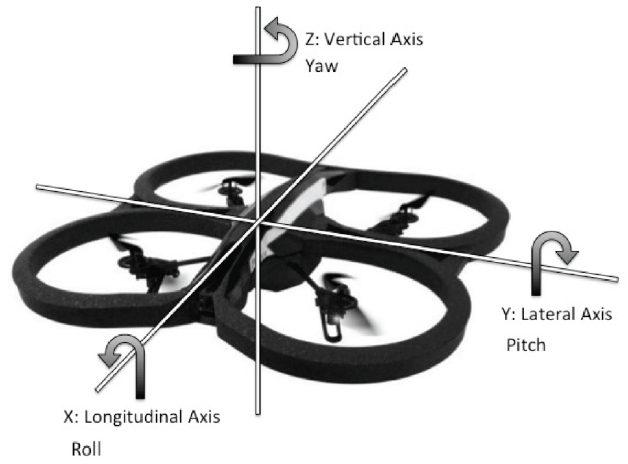
\includegraphics[scale=0.3]{pitch}
\caption{Pitch, yaw, and roll in the context of a quadcopter\cite{Hansen2014}}
\label{pitch}
\end{figure}
\end{aside}

\section{Results}
The reference physical deployment of octoDrone resulted in two programs (one for the base station, and another for the drones) running on three different pieces of hardware simultaneously. All of these units were able to communicate with each other and avoid collisions. The data that was ``collected'' (synthesised) was relayed to the base station in a timely manner. Finally, both of the drones were able to takeoff, move, and land according to plan, with minimal drift and disturbance from environmental factors.

\section{Review Against Original Objectives}
The objective from the specification in section \ref{sec:obj} was that ``The simulation code must be adaptable to the physical drones for real deployment''. This was most certainly achieved, and, in fact, exceeded in as much as the work that was done also outlines the procedure for adapting the simulator to arbitrary hardware platforms. It is probable that access to more expensive equipment would have streamlined the deployment process and improved the quality of the end result, but this is of little consequence in terms of a review against the specification.
